%===============================================================================
% LaTeX sjabloon voor de bachelorproef toegepaste informatica aan HOGENT
% Meer info op https://github.com/HoGentTIN/bachproef-latex-sjabloon
%===============================================================================

\documentclass{bachproef-tin}

\usepackage{hogent-thesis-titlepage} % Titelpagina conform aan HOGENT huisstijl
\usepackage[utf8]{inputenc}
\usepackage{glossaries}
\makeglossaries
\newglossaryentry{dansen}{name={dansen},description={jajajajaja}}
%%---------- Documenteigenschappen ---------------------------------------------
% TODO: Vul dit aan met je eigen info:

% De titel van het rapport/bachelorproef
\title{De impact van de transformatie van monolitische systemen naar microservices}

% Je eigen naam
\author{Joery Haelewyck}

% De naam van je promotor (lector van de opleiding)
\promotor{Giselle Vercauteren}

% De naam van je co-promotor. Als je promotor ook je opdrachtgever is en je
% dus ook inhoudelijk begeleidt (en enkel dan!), mag je dit leeg laten.
\copromotor{Yentl Verhelst en Alexander Sels }

% Indien je bachelorproef in opdracht van/in samenwerking met een bedrijf of
% externe organisatie geschreven is, geef je hier de naam. Zoniet laat je dit
% zoals het is.
\instelling{---}

% Academiejaar
\academiejaar{2020-2021}

% Examenperiode
%  - 1e semester = 1e examenperiode => 1
%  - 2e semester = 2e examenperiode => 2
%  - tweede zit  = 3e examenperiode => 3
\examenperiode{3}

%===============================================================================
% Inhoud document
%===============================================================================

\begin{document}

%---------- Taalselectie -------------------------------------------------------
% Als je je bachelorproef in het Engels schrijft, haal dan onderstaande regel
% uit commentaar. Let op: de tekst op de voorkaft blijft in het Nederlands, en
% dat is ook de bedoeling!

%\selectlanguage{english}

%---------- Titelblad ----------------------------------------------------------
\inserttitlepage

%---------- Samenvatting, voorwoord --------------------------------------------
\usechapterimagefalse
%%=============================================================================
%% Voorwoord
%%=============================================================================

\chapter*{\IfLanguageName{dutch}{Woord vooraf}{Preface}}
\label{ch:voorwoord}

%% TODO:
%% Het voorwoord is het enige deel van de bachelorproef waar je vanuit je
%% eigen standpunt (``ik-vorm'') mag schrijven. Je kan hier bv. motiveren
%% waarom jij het onderwerp wil bespreken.
%% Vergeet ook niet te bedanken wie je geholpen/gesteund/... heeft

De structuur van microservices wint aan belang in het bedrijfsleven. Dit is ook het geval bij TUI.
Bij deze grootspeler in de toeristische sector werk ik ondertussen 6 jaar: de eerste 3 jaar als backend developer en tot heden als frontend developer. TUI is ook bezig met de overschakeling van een monolithische architectuur naar een systeem bestaande uit microservices.\\
Deze verandering loopt niet zo vlot als initieel gedacht. Dit bracht me tot het idee om een onderzoek uit te voeren naar welke impact deze omschakeling uiteindelijk met zich meebrengt. In theorie zijn er veel voordelen verbonden aan microservices, meer dan bij een monolithische structuur. In de praktijk daarentegen wegen de baten niet altijd door. Door dit onderzoek heb ik nu een beter beeld over hoe deze architecturen precies werken en kan ik deze kennis toepassen in het werkleven.\\  
Graag wil ik mijn co-promotors, \textbf{Yentl Verhelst} en \textbf{Alexander Sels}, bedanken voor hun begeleiding en ondersteuning. Vervolgens wil ik ook mijn promotor, \textbf{Giselle Vercauteren}, bedanken voor de opvolging en controle van mijn onderzoek. Tenslotte hoop ik dat ik de mensen die mijn werk nalezen iets kan bijleren over mijn onderwerp.

%%=============================================================================
%% Samenvatting
%%=============================================================================

% TODO: De "abstract" of samenvatting is een kernachtige (~ 1 blz. voor een
% thesis) synthese van het document.
%
% Deze aspecten moeten zeker aan bod komen:
% - Context: waarom is dit werk belangrijk?
% - Nood: waarom moest dit onderzocht worden?
% - Taak: wat heb je precies gedaan?
% - Object: wat staat in dit document geschreven?
% - Resultaat: wat was het resultaat?
% - Conclusie: wat is/zijn de belangrijkste conclusie(s)?
% - Perspectief: blijven er nog vragen open die in de toekomst nog kunnen
%    onderzocht worden? Wat is een mogelijk vervolg voor jouw onderzoek?
%
% LET OP! Een samenvatting is GEEN voorwoord!

%%---------- Nederlandse samenvatting -----------------------------------------
%
% TODO: Als je je bachelorproef in het Engels schrijft, moet je eerst een
% Nederlandse samenvatting invoegen. Haal daarvoor onderstaande code uit
% commentaar.
% Wie zijn bachelorproef in het Nederlands schrijft, kan dit negeren, de inhoud
% wordt niet in het document ingevoegd.

\IfLanguageName{english}{%
\selectlanguage{dutch}
\chapter*{Samenvatting}



}{}

%%---------- Samenvatting -----------------------------------------------------
% De samenvatting in de hoofdtaal van het document

\chapter*{\IfLanguageName{dutch}{Samenvatting}{Abstract}}

De overgang van een monolithische architectuur naar een microservice-architectuur is een heuze onderneming. Veel bedrijven willen inspringen op de trend van microservices maar verliezen daarbij cruciale elementen uit het oog. Niet elk bedrijf is gebaat met een architectuur bestaande uit microservices, vooral kleinere ondernemingen hebben deze complexe vorm van architectuur niet nodig.
In dit onderzoek wordt er informatie verzameld omtrent de monolithische en microservice-architectuur. De voordelen en uitdagingen van deze architectuurvormen worden overlopen en in detail geanalyseerd. Vervolgens worden de twee systemen met elkaar vergeleken en wordt de focus gelegd op welke voordelen een transformatie naar microservices biedt. 

Een dergelijke transformatie wijzigt niet enkel de architectuur vorm, maar heeft ook impact op de dagelijkse werking van het bedrijf. Het personeel moet zich aanpassen, omgeschoold worden en sommige individuen verlaten de onderneming. De kosten zijn aanzienlijk. Hoe groter de monoliet, hoe meer tijd nodig is om de services los te koppelen van het systeem en om te zetten naar zelfstandige microservices. 

Er wordt een model opgesteld die helpt bij het aanduiden van de elementen die het meeste zullen veranderen door deze transformatie. De focus van het model ligt op het financiële en de sociale elementen van de onderneming.

Het model wordt toegepast op de situatie van TUI, een bedrijf die al enkele jaren bezig is met de transformatie van een monolithische architectuur naar microservices. Hieruit zal blijken dat een transformatie niet altijd het gewenste resultaat heeft. 

De conclusie is dat niet elke transformatie een succesverhaal zal zijn. Hoe beter het voorbereidend werk, hoe hoger de kans op slagen.



%---------- Inhoudstafel -------------------------------------------------------
\pagestyle{empty} % Geen hoofding
\tableofcontents  % Voeg de inhoudstafel toe
\cleardoublepage  % Zorg dat volgende hoofstuk op een oneven pagina begint
\pagestyle{fancy} % Zet hoofding opnieuw aan

%---------- Lijst figuren, afkortingen, ... ------------------------------------

% Indien gewenst kan je hier een lijst van figuren/tabellen opgeven. Geef in
% dat geval je figuren/tabellen altijd een korte beschrijving:
%
%  \caption[korte beschrijving]{uitgebreide beschrijving}
%
% De korte beschrijving wordt gebruikt voor deze lijst, de uitgebreide staat bij
% de figuur of tabel zelf.

\listoffigures
\printglossary
\printglossaries
% Als je een lijst van afkortingen of termen wil toevoegen, dan hoort die
% hier thuis. Gebruik bijvoorbeeld de ``glossaries'' package.
% https://www.overleaf.com/learn/latex/Glossaries

%---------- Kern ---------------------------------------------------------------

% De eerste hoofdstukken van een bachelorproef zijn meestal een inleiding op
% het onderwerp, literatuurstudie en verantwoording methodologie.
% Aarzel niet om een meer beschrijvende titel aan deze hoofstukken te geven of
% om bijvoorbeeld de inleiding en/of stand van zaken over meerdere hoofdstukken
% te verspreiden!

%%=============================================================================
%% Inleiding
%%=============================================================================

\chapter{\IfLanguageName{dutch}{Inleiding}{Introduction}}
\label{ch:inleiding}

Microservices is een architectuur die steeds populairder wordt. Bedrijven beginnen steeds meer over te schakelen naar deze structuur. Bestaande ondernemingen vertrekken meestal vanuit een monolithische architectuur. De transformatie van een monoliet naar microservices is een proces vol uitdagingen. Er zijn verschillende manieren om deze verandering tot stand te brengen. De focus van dit onderzoek ligt echter op de impact die een dergelijke transformatie met zich meebrengt.\\

De monolitische architectuur in software ontwikkeling betekent dat de programma's, applicaties, \emph{deployment}, interface, ... 1 geheel vormen. Voor startende ondernemingen en hoofdzakelijk kleine bedrijven is deze architectuur vaak voldoende om aan de noden van het bedrijf te voldoen.\\

Een groot nadeel van de monolieten is de schaalbaarheid. Het is moeilijk om individuele componenten uit te breiden. Hoe groter de monoliet, hoe complexer het systeem. Het wordt moeilijker om aanpassingen door te voeren, de instaptijd van nieuwe ontwikkelaars wordt langer en het zorgt ervoor dat het bedrijf minder flexibel kan reageren op marktsveranderingen.\\

De microservice architectuur biedt een oplossing voor deze problemen, waardoor bedrijven geneigd zijn om de overschakeling te maken. Terwijl een monolithische applicatie een enkele verenigde eenheid is, zal een applicatie bestaande uit microservices het geheel opsplitsen in een verzameling van kleinere onafhankelijke eenheden. Deze architectuur zorgt voor meer flexibiliteit omdat de componenten onafhankelijk \emph{gedeployed} kunnen worden. Het zorgt er ook voor dat de applicaties makkelijker uit te breiden zijn. \\

Naast alle voordelen die microservices biedt, brengt het ook wat uitdagingen met zich mee. Het systeem wordt complexer en mits alle componenten onafhankelijk werken, zorg dit voor een groter druk op de \emph{load balancer}.

\section{\IfLanguageName{dutch}{Probleemstelling}{Problem Statement}}
\label{sec:probleemstelling}

De belangrijkste doelgroep van dit onderzoek, zijn de bedrijven die willen overschakelen van een monolitische architectuur naar microservices. Het onderzoek kan ook een meerwaarde hebben voor personen die meer kennis willen verzamelen omtrent deze architecturen. 

\section{\IfLanguageName{dutch}{Onderzoeksvraag}{Research question}}
\label{sec:onderzoeksvraag}

Het doel van dit onderzoek is om te weten te komen wat de precieze impact is wanneer een bedrijf overschakelt van een monolitische architectuur naar een architectuur bestaande uit microservices.

De 3 hoofdvragen van dit onderzoek zijn als volgt:
\begin{itemize}
    \item Wat zijn de gevolgen van de transformatie?
    \item Wat zijn de financiële kosten die gemaakt worden tijdens de transformatie?
    \item Welk effect heeft deze transformatie op het sociale aspect van het bedrijf?
\end{itemize}

\section{\IfLanguageName{dutch}{Onderzoeksdoelstelling}{Research objective}}
\label{sec:onderzoeksdoelstelling}

Gebaseerd op de onderzoeksvragen die terug te vinden zijn in de vorige paragraaf. Wordt het volgende resultaat verwacht:

\begin{itemize}
    \item Een literatuurstudie omtrent microservices en de monolitische architectuur in software ontwikkeling. Waarin de voordelen en uitdagingen aangehaald worden.
    \item Een vergelijking tussen de twee architecturen. 
    \item Een model die als basis dient om een schatting te maken van de impact.
    \item Het model toepassen op een hedendaagse bedrijfssituatie.
\end{itemize}
Naast alle voordelen die microservices biedt, brengt het ook wat uitdagingen met zich mee. Het systeem wordt complexer en mits alle componenten onafhankelijk werken, zorg dit voor een groter druk op de \emph{load balancer}.

\section{\IfLanguageName{dutch}{Probleemstelling}{Problem Statement}}
\label{sec:probleemstelling}

De belangrijkste doelgroep van dit onderzoek, zijn de bedrijven die willen overschakelen van een monolithische architectuur naar microservices. Het onderzoek kan ook een meerwaarde hebben voor personen die meer kennis willen verzamelen omtrent deze architecturen. 

\section{\IfLanguageName{dutch}{Onderzoeksvraag}{Research question}}
\label{sec:onderzoeksvraag}

Het doel van dit onderzoek is om te weten te komen wat de precieze impact is wanneer een bedrijf overschakelt van een monolithische architectuur naar een architectuur bestaande uit microservices.

De 3 hoofdvragen van dit onderzoek zijn als volgt:
\begin{itemize}
    \item Wat zijn de gevolgen van de transformatie?
    \item Wat zijn de financiële kosten die gemaakt worden tijdens de transformatie?
    \item Welk effect heeft deze transformatie op het sociale aspect van het bedrijf?
\end{itemize}

\section{\IfLanguageName{dutch}{Onderzoeksdoelstelling}{Research objective}}
\label{sec:onderzoeksdoelstelling}

Gebaseerd op de onderzoeksvragen die terug te vinden zijn in de vorige paragraaf. Wordt het volgende resultaat verwacht:

\begin{itemize}
    \item Een literatuurstudie omtrent microservices en de monolithische architectuur in software ontwikkeling. Waarin de voordelen en uitdagingen aangehaald worden.
    \item Een vergelijking tussen de twee architecturen. 
    \item Een model die als basis dient om een schatting te maken van de impact.
    \item Het model toepassen op een hedendaagse bedrijfssituatie.
\end{itemize}

\section{\IfLanguageName{dutch}{Opzet van deze bachelorproef}{Structure of this bachelor thesis}}
\label{sec:opzet-bachelorproef}

% Het is gebruikelijk aan het einde van de inleiding een overzicht te
% geven van de opbouw van de rest van de tekst. Deze sectie bevat al een aanzet
% die je kan aanvullen/aanpassen in functie van je eigen tekst.

De rest van deze bachelorproef is als volgt opgebouwd:

In Hoofdstuk 2 wordt een over--zicht gegeven van de stand van zaken binnen het onderzoeksdomein, op basis van een literatuurstudie.

In Hoofdstuk \ref{ch:methodologie} wordt de methodologie toegelicht en worden de gebruikte onderzoekstechnieken besproken om een antwoord te kunnen formuleren op de onderzoeksvragen.

In Hoofdstuk \ref{ch:model} wordt het model opgebouwd die als basisstuk dient om de schatting te maken van de impact van de transformatie.

In Hoofdstuk \ref{ch:usecase} passen we het model toe op een bedrijf die momenteel een monolithische architectuur gebruikt en overschakelt naar een architectuur bestaande uit microservices.
--
\section{\IfLanguageName{dutch}{Opzet van deze bachelorproef}{Structure of this bachelor thesis}}
\label{sec:opzet-bachelorproef}

% Het is gebruikelijk aan het einde van de inleiding een overzicht te
% geven van de opbouw van de rest van de tekst. Deze sectie bevat al een aanzet
% die je kan aanvullen/aanpassen in functie van je eigen tekst.

De rest van deze bachelorproef is als volgt opgebouwd:

In Hoofdstuk~\ref{ch:stand-van-zaken} wordt een over--zicht gegeven van de stand van zaken binnen het onderzoeksdomein, op basis van een literatuurstudie.

In Hoofdstuk~\ref{ch:methodologie} wordt de methodologie toegelicht en worden de gebruikte onderzoekstechnieken besproken om een antwoord te kunnen formuleren op de onderzoeksvragen.

In Hoofdstuk \ref{ch:model} wordt het model opgebouwd die als basisstuk dient om de schatting te maken van de impact van de transformatie.

In Hoofdstuk \ref{ch:usecase} passen we het model toe op een bedrijf die momenteel een monolitische architectuur gebruikt en overschakelt naar een architectuur bestaande uit microservices.

% TODO: Vul hier aan voor je eigen hoofstukken, één of twee zinnen per hoofdstuk

In Hoofdstuk~\ref{ch:conclusie}, tenslotte, wordt de conclusie gegeven en een antwoord geformuleerd op de onderzoeksvragen. Daarbij wordt ook een aanzet gegeven voor toekomstig onderzoek binnen dit domein.
\label{ch:stand-van-zaken}
\graphicspath{{./img/}}
% Tip: Begin elk hoofdstuk met een paragraaf inleiding die beschrijft hoe
% dit hoofdstuk past binnen het geheel van de bachelorproef. Geef in het
% bijzonder aan wat de link is met het vorige en volgende hoofdstuk.

% Pas na deze inleidende paragraaf komt de eerste sectiehoofding.
\chapter{Stand van zaken}
\textbf{Inleiding}

In dit hoofdstuk wordt de huidige toestand van monolithische en microservice-architectuur besproken. De focus ligt hoofdzakelijk op het deel van microservices omdat de eindtoestand van de transformatie voor dit onderzoek het belangrijkst is.

\section{Microservice-architectuur}

\subsection{Service oriented architecture}
De term Service Oriented Architecture of SOA wordt vaak vermeld tijdens het bespreken van microservices. De twee architecturen hebben heel wat gemeenschappelijk maar er zijn toch wat verschillen. Om die reden wordt er eerst uitgeklaard wat deze verschillen zijn en welke aspecten de architecturen delen. 

Het onderzoek van Vieira ~\autocite{Vieira2019} leert ons dat SOA een manier definieert om softwarecomponenten herbruikbaar te maken via service-interfaces. Deze interfaces maken gebruik van gemeenschappelijke communicatiestandaarden. Hierdoor is het mogelijk om de services snel op te nemen in nieuwe applicaties zonder elke keer een zware integratie uit te voeren. 

Iedere service vertegenwoordigt een business gerelateerd aspect. De service bevat de code en de nodige gegevensintegraties om het functionele aspect volledig en zelfstandig uit te voeren, bijvoorbeeld het afhandelen van een betaling.\\

\begin{figure}[!htb]
    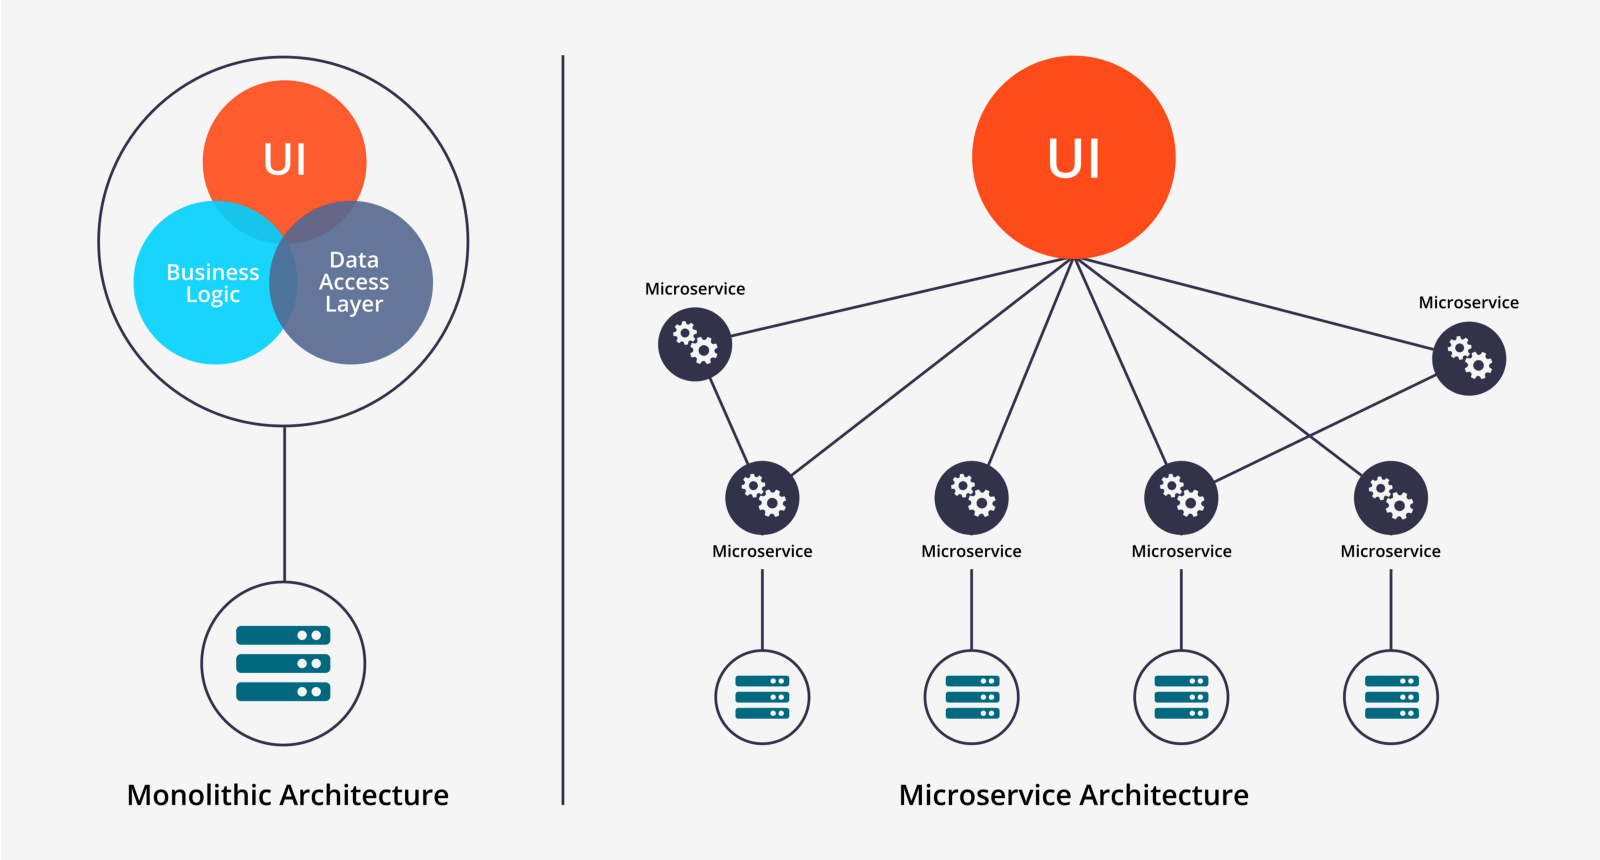
\includegraphics[width=0.95\textwidth]{Microservices_vs_mono.png}
    \caption{Grafische vergelijking tussen een monoliet en microservices \label{microvsmono}}
    \centering

\end{figure}

De service-interfaces zorgen voor een losse koppeling waardoor ze aangesproken kunnen worden met weinig of geen kennis van het onderliggend systeem. De services worden weergegeven met behulp van de standaard netwerkprotocollen zoals SOAP.

Ten opzichte van de standaard architecturen die SOA voorgingen (zoals de monoliet), biedt het tal van voordelen:
\begin{itemize}
     \item \textbf{Flexibiliteit}: De mogelijkheid om componenten te hergebruiken zorgt ervoor dat een onderneming zich flexibeler kan opstellen en sneller kan reageren op marktsveranderingen. 
     \item \textbf{De mogelijkheid om legacy functionaliteit te integreren in nieuwe markten}: SOA biedt de mogelijkheid om functionaliteit van oude systemen te integreren naar nieuwe systemen.
     \item \textbf{Een betere connectie tussen IT en business}: In een SOA architectuur kunnen de services gedefinieerd worden als business termen. Hierdoor kunnen de analisten efficiënter werken en sneller de developers aanspreken. De scope van de services zijn ook makkelijker te definiëren.
\end{itemize} 

Veel experten beweren dat de microservices-architectuur de volgende stap is in de evolutie van SOA of dat het de correctie implementatie is van SOA. Er zijn tal van studies die deze twee architecturen vergelijken, maar voor dit onderzoek bespreken we enkel het verschil tussen de scope en de koppeling van de componenten. \autocite{Education2019}


SOA is een ondernemingsbreed concept. Het maakt het mogelijk om bestaande applicaties weer te geven via los gekoppelde interfaces, die elk verantwoordelijk zijn voor een bedrijfsfunctie, waardoor de applicaties een onderdeel vormen van een groot geheel. Vaak zijn deze componenten verbonden aan de hand van een integratie bus.

Microservices-architectuur is een concept met toepassingsbereik. Het splitst de applicatie op in kleine onderdelen die onafhankelijk gewijzigd, geschaald en beheerd kunnen worden. Het definieert niet hoe applicaties met elkaar communiceren.
\begin{figure}[!htb]
    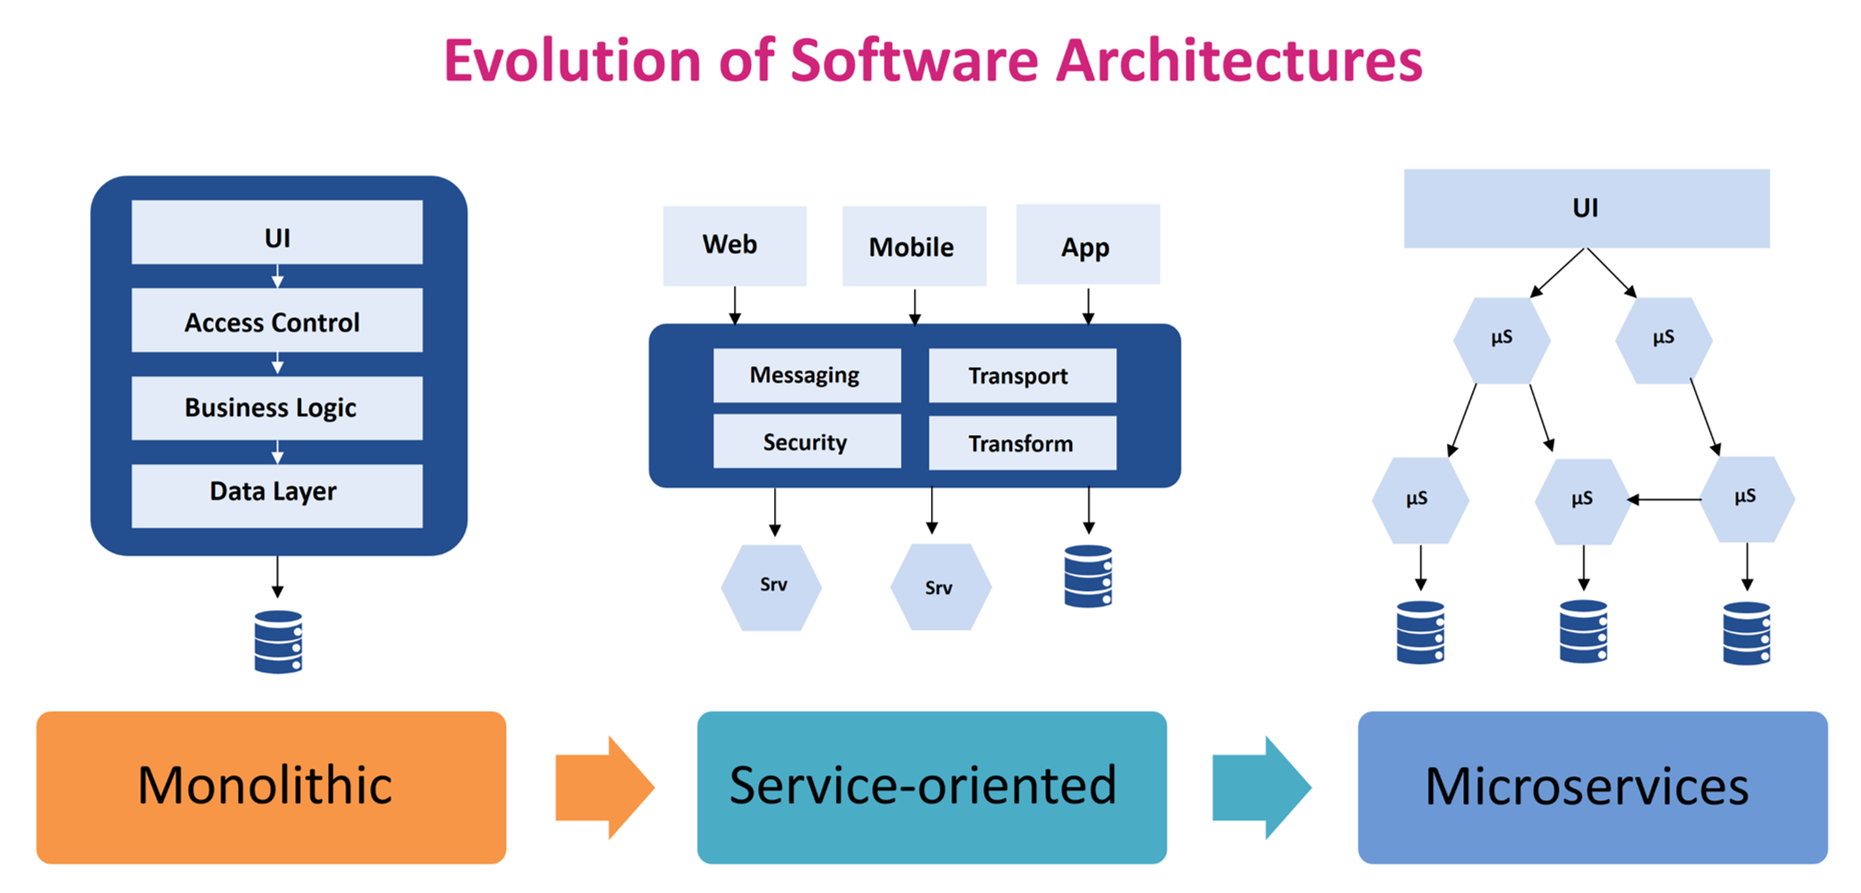
\includegraphics[width=1\textwidth]{Evolution-of-Software-architectur.png}
    \caption{Evolutie van software architectuur \label{evolution}}
\end{figure}


\subsection{Voordelen}
Om de impact in te schatten van de transformatie is het belangrijk dat de voordelen van een microservice architectuur gekend zijn. Om een algemene opsomming te vermijden en meer structuur te brengen in deze lijst, worden de voordelen onderverdeeld in 3 categorieën . In eerste instantie worden de voordelen besproken die horen bij het \underline{design} van mircoservices, vervolgens komt het gedeelte van de \underline{development} aan bod en tenslotte de \underline{deployment}.\\

\textbf{Design}\\ 
Tijdens het design van een microservice-architectuur kunnen er al tal van voordelen genoteerd worden. Het ontwikkelen van deze architectuur zorgt ervoor dat men stil staat bij de scope van het project.\\ 
Een goed afgebakend project geeft een goed overzicht van de noden weer. Veel microservices maken gebruik van Cloud native computing wat meer flexibiliteit biedt. Microservices passen gedecentraliseerd beheer toe, wat betekent dat het development team de code kan ontwikkelen volgens hun individuele beheersplannen.\\ 
Het systeem zal ook zodanig ontwikkeld worden dat wanneer een component uitvalt het systeem verder blijft werken. Deze eigenschap heet fouttolerantie. Een bijhorende patroon is het gebruik van een 'circuit breaker'. Deze service handelt fouten af die ontstaan bij het aanspreken van andere services.\\
Iedere service bevat zijn eigen database. Dit helpt mee aan de 'loosely coupled' strategie, veranderingen aan één database beïnvloeden de andere databases niet.\\
Services met gemeenschappelijke doeleinden kunnen gegroepeerd worden, hierdoor ontstaan 'lagen' van
componenten. Dit biedt de mogelijkheid om logica te hergebruiken en te isoleren.\\ \\
\textbf{Development}\\ Eén van de grote voordelen van het ontwikkelen van microservices is dat developers zich kunnen concentreren op één service per keer. Ze hebben de vrijheid om te kiezen welke technologie ze willen gebruiken. Het is perfect mogelijk om 10 verschillende componenten in 10 verschillende technologieën te ontwikkelen. Natuurlijk moet er een consensus zijn over wat er wel of niet gebruikt mag worden. Bepaalde logica kan hergebruikt worden in meerdere services of een service kan verschillende componenten voeden waardoor veel werk herbruikbaar is. \\
Het ontwikkelen van integratietesten gaat ook sneller dankzij de kleinschalige componenten. Dependenties met andere services kunnen makkelijk opgevangen worden met Mocks.\\
\textbf{Deployment}\\ Door gebruik te maken van microservices kan een onderneming kiezen om meerdere pipelines te gebruiken om een project in productie te plaatsen. Een pipeline per services is geen uitzondering. Hierdoor is de CI/CD van het project veel robuuster en zijn fouten sneller op te lossen.

\begin{figure}[!htb]
    \centering
    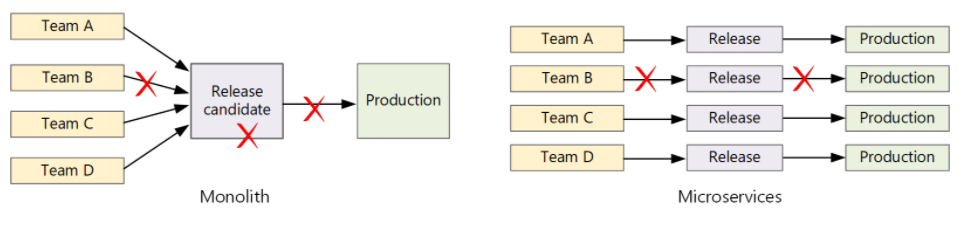
\includegraphics[width=0.9\textwidth]{PipelinesVS.png}    
    \caption{grafische vergelijking tussen het release proces van een monoliet en microservices \label{pipelin}}
\end{figure}

Het beheer van de code wordt ook een stuk eenvoudiger. Het uitvoeren van updates kan beter beheerd worden en geïsoleerd worden van componenten die de update niet nodig hebben. Rollbacks zijn beperkter en hebben enkel impact op bepaalde services.


\subsection{Pijnpunten}

Elke software architectuur heeft zijn uitdagingen of pijnpunten. Voor microservices is dit niet anders. Net zoals in sectie 2.1.2 verdelen we de nadelen op in 3 categorieën: \underline{design}, \underline{development} en \underline{deployment}.\\ \\

\textbf{Design} \\De API die geleverd wordt door een microservice wordt een soort contract tussen degelijke microservices en degenen die de API consumeren. Deze contracten zijn bindend en mogen niet geschonden worden. Dit heeft een negatieve impact op de versiebeheer van de API's geleverd door de microservices.\\    Toegangscontrole kan snel uit de hand lopen bij microservices. Elke service heeft zijn eigen noden en veel tools bieden enkel een gecentraliseerd beheer van accounts aan.\\    Microservices stellen meer API's bloot en distribueren authenticatie en toegangscontrole. Het oppervlak dat kwetsbaar is, is dus veel uitgebreider en dit is de belangrijkste reden waarom proliferatie van eindpunten significant wordt herkend als een pijnpunt door industriële onderzoekers en praktijkmensen.\\  \\
\textbf{Development} \\ Als de opslagruimte gedeeld moet worden tussen de verschillende microservices, wordt het lastig om gegevensconsistentie te waarborgen. Dit is zeker het geval wanneer gevoelige data zoals contactgegevens gebruikt wordt over meerdere services.\\
Door de technische heterogeniteit kunnen verschillende technologieën gebruikt worden. Indien dit het geval is, dan is er een team van bekwame medewerkers nodig om de grote heterogene gedistribueerde software te ondersteunen. Dit brengt een grote financiële kost met zich mee.\\
Het development team kan geografisch verspreid zijn. Componenten van de applicatie kunnen dus beheerd worden in verschillende landen. Dit bemoeilijkt de communicatie en vertraagt het ontwikkelingsproces.\\
De communicatie tussen de verschillende services gebeurdt over een netwerk. Dit zorgt ervoor dat de services afhankelijk zijn van dit netwerk.\\ \\
\textbf{Deployment} \\ Elke service zal zelf een logboek bijhouden, hierdoor moet er een extra service gecreëerd worden om alles logs te verzamelen in een overzicht.\\
De grootte en complexiteit van het implementatieproces kan voor sommige bedrijven een obstakel vormen.

\subsection{Toepassingen en design patterns}

Er zijn heel wat design patterns die gebruikt kunnen worden om de microservice architectuur te verwezelijken, zie figuur \ref{overzicht} . Om de scope van deze studie te beperken zullen we ze niet allemaal behandelen. Het werk van Richardson ~\autocite{Richardson2021} werd gebruikt als inspiratiebron.\\ \\
\textbf{Aggregator Pattern}\\
Aggregator verwijst naar een website of programma dat gerelateerde gegevens verzamelt en weergeeft. In Microservices-patronen is Aggregator een basiswebpagina die verschillende services oproept om de vereiste informatie te verkrijgen of om de correcte functionaliteit aan te bieden.\\
Het Aggregate Design Pattern is gebaseerd op het DRY-principe. Op basis van dit principe wordt de logica geabstraheerd in samengestelde microservices om daarna deze specifieke bedrijfslogica samen te voegen tot één service. ~\autocite{Kappaggantula2020} \\
Bijvoorbeeld: twee services A en B kunnen afzonderlijk gelijktijdig geschaald worden door de gegevens aan de samengestelde microservice te verstrekken, zie figuur ~\ref{aggragator} . \\ \\

\begin{figure}[!htb]
    \centering
    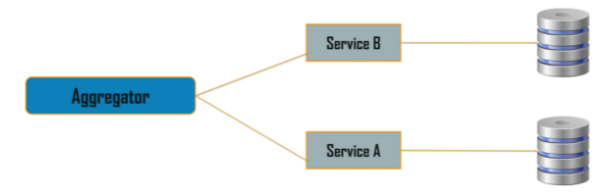
\includegraphics[width=1\textwidth]{Aggregator.png}
    \caption{Aggragator Pattern \label{aggragator}}
\end{figure}

\textbf{Strangler Pattern}\\
De strangler pattern is een manier om een legacy systeem stapsgewijs te migreren door bestaande functionaliteiten te vervangen door nieuwe applicaties en diensten in een gefaseerde aanpak. Over tijd zal het nieuwe systeem alle functionaliteit van het oude systeem bevatten en bijgevolg het systeem vervangen, zie figuur ~\ref{stangler} .

\begin{figure}[!htb]
    \centering
    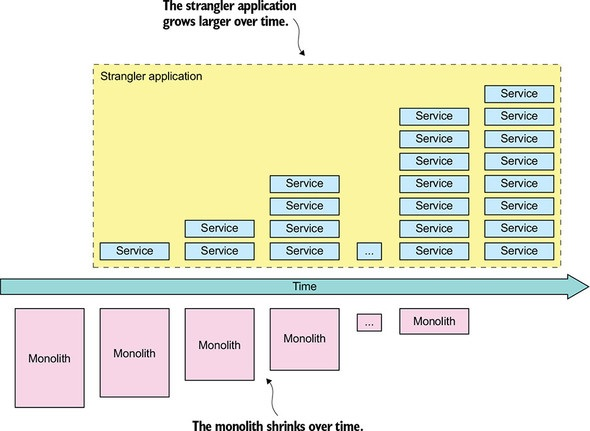
\includegraphics[height=8cm]{strangler.jpg}
    \caption{Straggler Pattern \label{stangler}}
\end{figure}

\textbf{Saga Pattern}
\\Een saga is een opeenvolging van lokale transacties. Elke lokale transactie werkt de database bij en publiceert een bericht of gebeurtenis om de volgende lokale transactie in de saga te activeren. Als een lokale transactie mislukt, voert de saga een rollback uit.\\
Dit patroon is toepasbaar wanneer elke service over zijn eigen database beschikt, zie figuur ~\ref{Saga} . \\ \\

\begin{figure}[!htb]
    \centering
    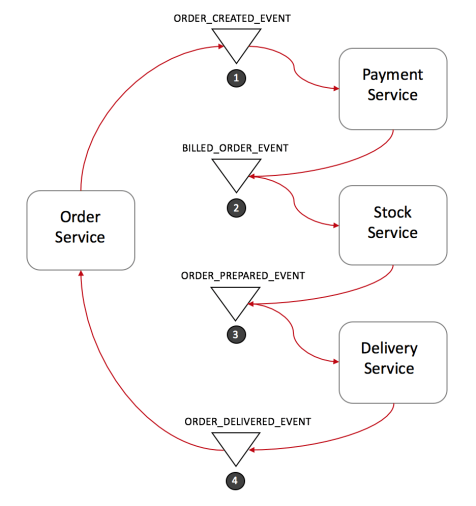
\includegraphics[height=10cm]{Saga.png}
    \caption{Saga Pattern \label{Saga}}
\end{figure}

\textbf{Circuit Breaker}\\
Het idee achter de 'Circuit Breaker' is relatief eenvoudig. Net zoals een elektrische stroomonderbreker zal de service tijdelijk uitgeschakeld worden als er te veel fouten geregistreerd worden. In deze periode zullen alle pogingen om de service aan te roepen mislukken. Na deze periode zal de 'stroomonderbreker' een aantal verzoeken aanvaarden en controleren of de verzoeken slagen. Als deze controle succesvol is, wordt de service hervat, zo niet blijft de 'stroomonderbreker' actief.
Er zijn drie toestanden: gesloten, half-open en open. In de gesloten toestand werkt alles zoals het hoort, zie figuur~\ref{gesloten}. 

\begin{figure}[!htb]
    \centering
    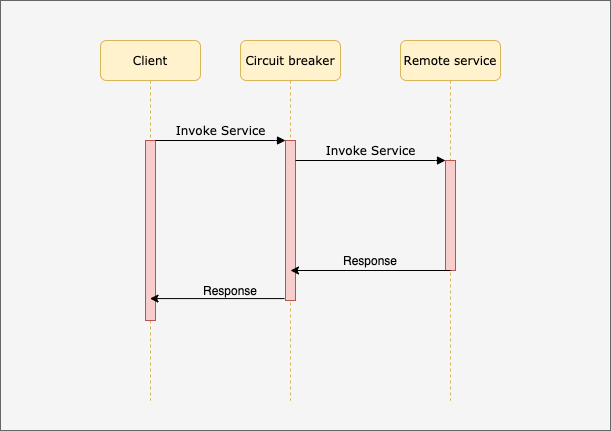
\includegraphics[height=10cm]{closed.png}
    \caption{Gesloten status \label{gesloten}}
\end{figure}

Zodra het aantal storingen een vooraf bepaalde drempel overschrijdt, schakelt de stroomonderbreker uit en gaat deze in de open toestand, zie figuur~\ref{open}.
\begin{figure}[!htb]
    \centering
    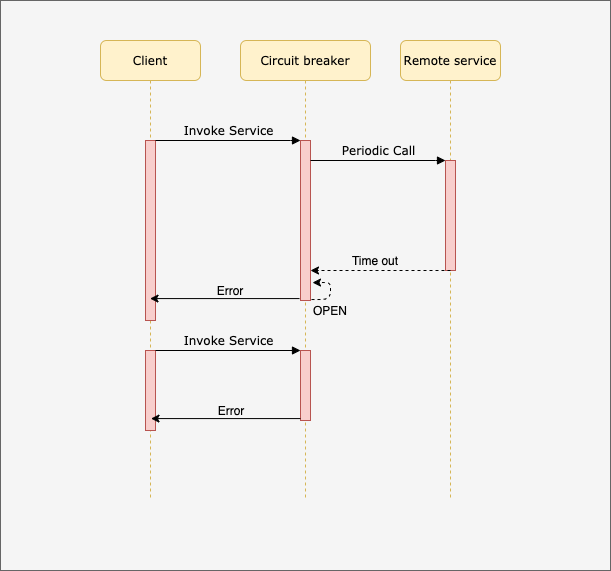
\includegraphics[height=10cm]{open.png}
    \caption{Open status \label{open}}
\end{figure}

Na een bepaalde tijd schakelt het circuit over naar een half-open toestand, zie figuur~\ref{halfopen}, om te testen of het onderliggende probleem nog steeds bestaat. De 'stroomonderbreker' gebruikt een mechanisme om periodiek een proefoproep te doen naar de externe service om te controleren of deze is hersteld. Als de oproep naar de externe service mislukt, blijft de stroomonderbreker in de open toestand. Als de oproep succesvol terugkeert, schakelt het circuit over naar de gesloten status. De vermogensschakelaar stuurt dan alle externe oproepen naar de service terug met een fout tijdens de half-open toestand.

\begin{figure}[!htb]
    \centering
    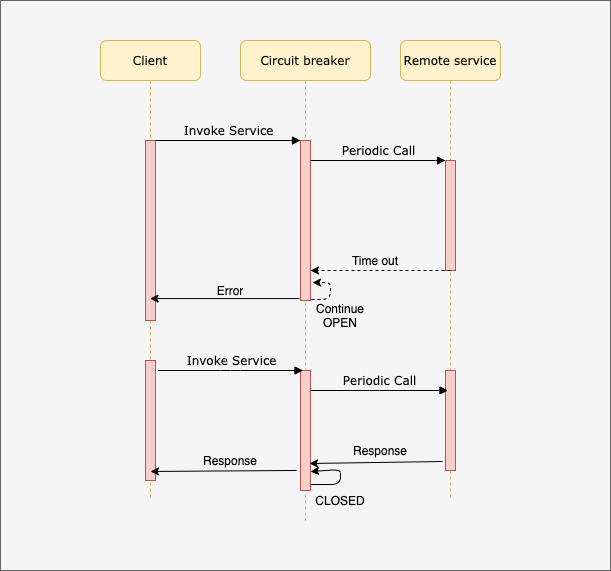
\includegraphics[height=10cm]{half-open.png}
    \caption{Half-open status \label{halfopen}}
\end{figure}

\textbf{Distributed Tracing}
Tracering is een fundamenteel proces in software-engineering, dat door programmeurs samen met andere vormen van registreren wordt gebruikt om informatie te verzamelen over het gedrag van een applicatie. Traditionele tracering stuit echter op problemen wanneer het wordt gebruikt om problemen op te lossen met applicaties die zijn gebouwd op een gedistribueerde softwarearchitectuur. Omdat microservices onafhankelijk schaalbaar zijn, is het gebruikelijk dat meerdere iteraties van een enkele service tegelijkertijd op verschillende servers, locaties en omgevingen worden uitgevoerd, waardoor een complex web ontstaat waar een verzoek doorheen moet. Deze verzoeken zijn bijna onmogelijk te volgen met traditionele technieken die zijn ontworpen voor een enkele servicetoepassing.
\\
Gedistribueerde traceringsoplossingen lossen dit probleem en tal van andere prestatieproblemen op, omdat het verzoeken via elke service of module kan volgen en een end-to-end narratief verslag van dat verzoek kan bieden. Analisten, SRE's, ontwikkelaars en anderen kunnen elke iteratie van een functie observeren, waardoor ze prestatiebewaking kunnen uitvoeren door te zien welke instantie van die functie ervoor zorgt dat de app vertraagt of faalt, en hoe ze dit kunnen oplossen. Zie figuur~\ref{distributed}

\begin{figure}[!htb]
    \centering
    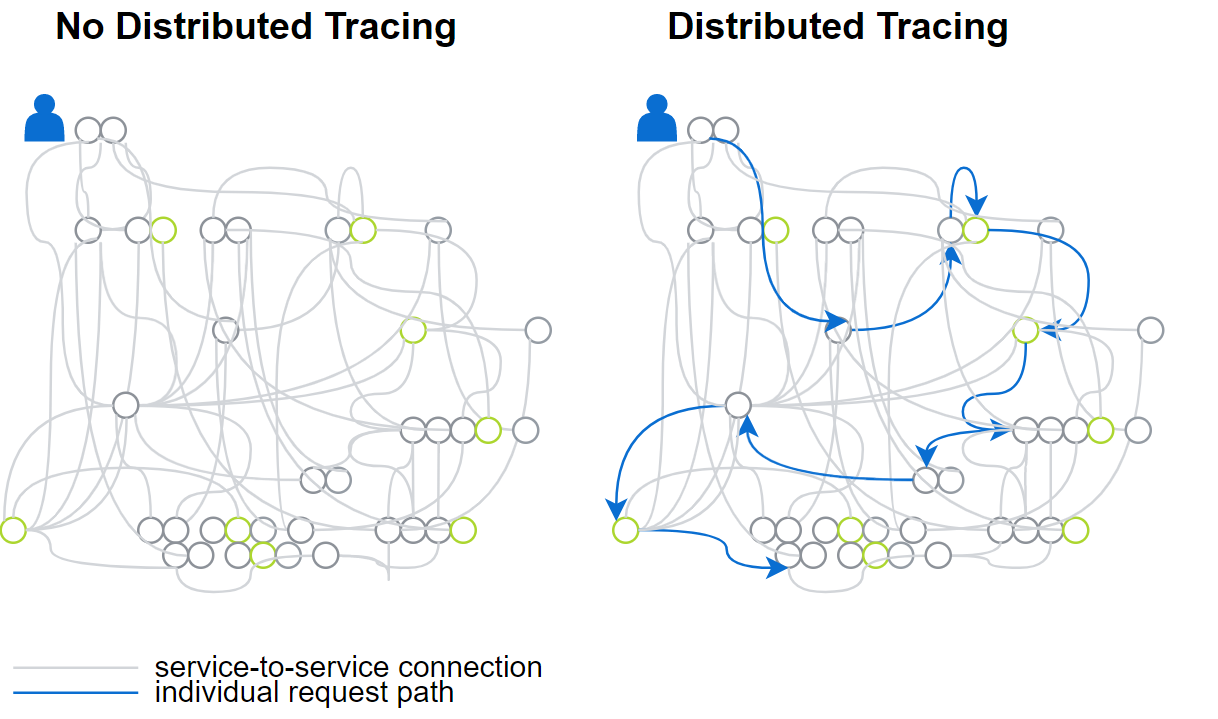
\includegraphics[height=10cm]{DistributedTracing.png}
    \caption{Distributed Tracing \label{distributed}}
\end{figure}
\begin{figure}[!htb]
    \centering
    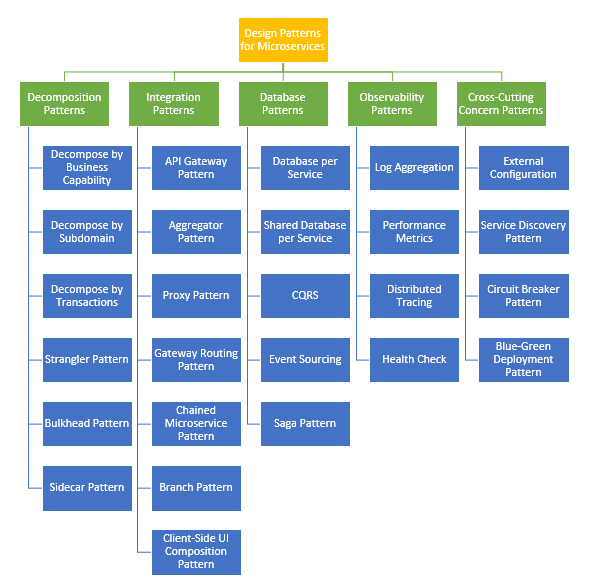
\includegraphics[height=10cm]{DesignPatterns.png}
    \caption{Overzicht Design Patterns \label{overzicht}}
\end{figure}
\newpage
\subsection{Micro Frontends}
Een volgende stap is om het concept van micro services toe te passen op de frontend. De huidige trend in web ontwikkeling zijn single page applicaties. De bekendste en meeste gebruikte SPA frameworks zijn React, Angular en Vue. In vele gevallen wordt de frontend onderhouden door één afzonderlijk team. Hierdoor groeit de frontend laag geleidelijk aan in een groot project, ook wel een frontend monoliet genoemd.\\\\
Het artikel van ~\autocite{Geers2020} leert ons dat het idee achter de micro frontends is om de website op te delen op basis van features en met behulp van compositie de verschillende delen samen te brengen in een werkende website. In theorie worden de features onderhouden door onafhankelijke teams. Elk team is verantwoordelijk voor zijn feature. De teams hebben een bepaald doel en dat doel is meestal gekoppeld aan een business requirement. Het team ontwikkelt alles zelfstandig, vanaf het moment de data opgehaald wordt uit de database  tot en met de user interface. In het verleden werden dergelijke benaderingen ‘frontend integratie voor verticale systemen’ genoemd. De benaming van microfront ends is eleganter, zie figuur ~\ref{microfrontends} .

De kernideeën achter Micro frontends:
\begin{itemize}
    \item \textbf{Team code is geïsoleerd} \\
          Elk team heeft zijn eigen stack en pipeline waar hun code gebouwd wordt. Afhankelijkheden op andere teams worden vermeden.
    \item \textbf{Elke team bepaalt hun eigen technologie} \\
          De teams hebben de vrijheid om de technologie te kiezen die zij wensen te gebruiken, zonder af te stemmen met andere teams. 
    \item \textbf{Teamvoorvoegsels instellen}\\
          Op plaatsen waar het niet mogelijk is om code te isoleren, moet het duidelijk zijn welk team eigenaar is van de niet geïsoleerde code. Dit kan gerealiseerd worden met naamgevingsconventies.  
    \item \textbf{Verkies browserfuncties boven aangepaste API’s}\\
          In eerste instantie worden browserfuncties gebruikt om te communiceren. Als deze functionaliteit ontoereikend is, kan er voor een aangepaste API geopteerd worden. 
    \item \textbf{Bouw een veerkrachtige website}
          Elke feature moet zijn nut hebben. Als dit niet het geval is, moet de feature verwijderd worden of geabsorbeerd worden in een ander team.\\
\end{itemize}
\begin{figure}[!htb]
    \centering
    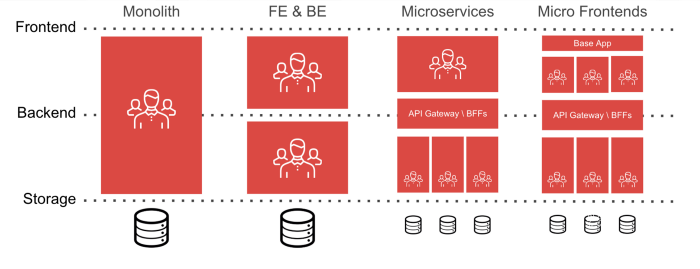
\includegraphics[height=10cm, width=15cm]{MicroFrontendsVertical.png}
    \caption{Evolutie naar micro frontends \label{microfrontends}}
\end{figure}

\newpage
\subsection{Mono- en polyrepo}
Wanneer alle code in één en dezelfde repository bijgehouden wordt, spreken we over een monorepo. De apps zijn dan onderverdeeld in verschillende subfolders. Deze structuur komt in veel projecten voor. Code in deze structuur heeft meestal één pipeline voor de implementatie. Dit zorgt voor een eenvoudige onderhoud, maar een enkele bug kan het hele proces vertragen.\\ 
Wanneer de code opgedeeld wordt in verschillende repositories, spreken we over een polyrepo. Een project is dan verspreid over meerdere bronnen. Dit heeft verscheidene voordelen maar brengt ook wat nadelen met zich mee.\\
Volgens het onderzoek van Powell ~\autocite{Powell2021} delen bedrijven die gebruik maken van microservices hun code op in verschillende repositories (polyrepos). De teams ontwikkelen hun services onafhankelijk van elkaar en bij gevolg gebruiken ze dus hun eigen repo. De voordelen van deze structuur zijn duidelijk. Een klein team kan snel en zonder restricties hun eigen code in productie plaatsen.\\  
Het nadeel is dat alle kennis verspreid is over verschillende repos, in het slechtste geval kom je op een punt waarbij niemand meer weet hoe het volledige systeem opgebouwd en geïmplementeerd wordt. Bij een slechte implementatie kunnen er ook \emph{dependencies} ontstaan tussen de verschillende repos. \\
\\
\\
\\
\\
Het gebruik van een enkele repo (monorepo) heeft enkele voordelen:
\begin{itemize}
    \item \textbf{Beter overzicht}\\
        Als een service gebruikt maakt van een andere service, zal het makkelijker zijn om te zien wat er precies in de code gebeurd. Bugs kunnen hierdoor sneller toegewezen worden aan een team.
    \item \textbf{Hergebruik van code}\\
        Er zal altijd gemeenschappelijke code zijn tussen verschillende services. Als het team kiest om deze code niet te dupliceren, is het makkelijker om in een monorepo de code te hergebruiken. Dit gaat wel in tegen het principe dat elke service onafhankelijk en geïsoleerd moet zijn.
    \item \textbf{Verbeterede samenwerking}\\
        Een enkele repository verwijdert de barrière tussen teams. Het zorgt voor meer toegankelijkheid. 
    \item \textbf{Standaardisatie}\\
        Het is eenvoudiger om code te standaardiseren en om een beleid te hanteren. Dit gaat natuurlijk weer in tegen de principes van mircoservices.
    \item \textbf{Refactoring}\\
        Het is minder werk om code structuren aan te passen in een enkele repository dan code die verspreidt is over meerder repositories.
    \item \textbf{Kennis}\\
        Alle logica is terug te vinden in enkele repo, hierdoor is er minder verlies van kennis over de jaren heen.
\end{itemize}
Een monorepo brengt ook wat uitdagingen met zich mee. Simpele aanpassingen in de code kan een grote impact hebben op andere componenten. Het implementatie proces is ingewikkelder en kan bij foute implementatie heel wat vertraging opleveren.\\ 
Beide strategieën hebben hun voor- en nadelen, er is geen winnaar. Het team kiest welk systeem het best aan zijn noden voldoet.

\newpage
\section{Monolithische architectuur}
Volgens de blog van Annett ~\autocite{Monolith2014} is een monolithische architectuur samengesteld is uit één stuk. De Monololitisch applicatie beschrijft een softwareapplicatie waarin verschillende componenten worden gecombineerd tot een enkel programma vanaf één enkel platform. De volgende componenten kunnen voorkomen:
\begin{itemize}
    \item Authorisatie
    \item Presentatie
    \item Business logica
    \item Database laag
    \item applicatie integratie
    \item notificatie module
\end{itemize}
\begin{figure}[!htb]
    \caption{Monolithische architectuur}
    \centering
    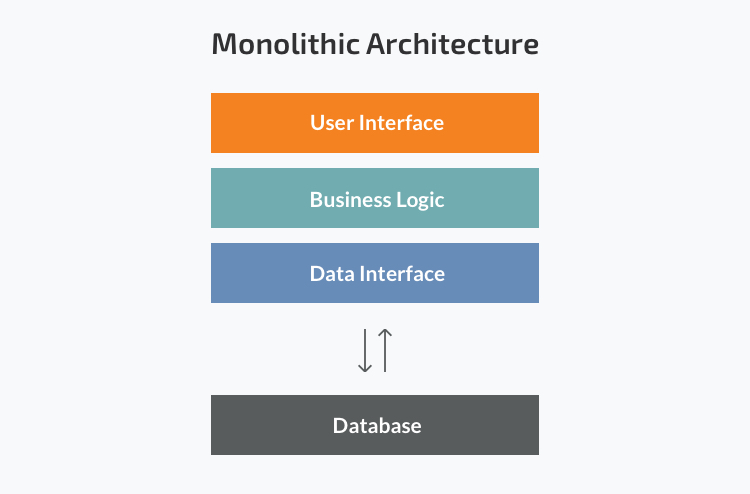
\includegraphics[width=1\textwidth]{Monoliet.png}
\end{figure}
Deze achitectuurvorm biedt de meeste voordelen bij kleinschalige projecten of systemen. Mits alles één geheel vormt, is een dergelijke applicatie makkelijk te ontwikkelen en ligt de progressiesnelheid relatief hoog. Hoe groter het project hoe meer problemen zich voordoen bij monolithische systemen. De codekwaliteit zal snel dalen als er meer duplicate code zal onstaan. Nieuwe features zullen trager ontwikkeld worden. Bugs zullen minder snel opgespoord worden. Een bijkomend probleem is dat nieuwe developers tijd zullen nodig hebben om in het project mee te stappen omdat de kennis hoofdzakelijk bij de originele ontwikkelaars zit. \\
Een nadeel is dat bij elke update het volledige deployprocess uitgevoerd wordt. Hierdoor is het onmogelijk om CI/CD te implementeren en wordt er meestal met een vast \emph{deploy} moment gewerkt. Als een update mislukt, moet het volledige systeem teruggedraaid worden.\\
De applicatie bevat in vele gevallen maar één technologie. Hierdoor is het systeem volledig afhankelijk van die ene technologie. Dit zorgt ervoor dat de onderneming minder snel op een marktsverandering kan inspelen.\\
Monolieten kunnen meestal enkel maar verticaal geschaald worden.

%%=============================================================================
%% Methodologie
%%=============================================================================

\chapter{\IfLanguageName{dutch}{Methodologie}{Methodology}}
\label{ch:methodologie}

%% TODO: Hoe ben je te werk gegaan? Verdeel je onderzoek in grote fasen, en
%% licht in elke fase toe welke stappen je gevolgd hebt. Verantwoord waarom je
%% op deze manier te werk gegaan bent. Je moet kunnen aantonen dat je de best
%% mogelijke manier toegepast hebt om een antwoord te vinden op de
%% onderzoeksvraag.

\lipsum[21-25]


%%=============================================================================
%% Model
%%=============================================================================

\chapter{\IfLanguageName{dutch}{Model}{Model}}
\label{ch:model}



\section{Inleiding}

In dit hoofdstuk behandelen we de elementen die impact ondervinden van een architectuur verandering, specifiek de transformatie van een monolithische architectuur naar microservices.

De elementen verdelen we op in twee categorieën. De eerste categorie bevat alle aspecten die te maken hebben met het financiële plaatje. Hieronder zullen elementen zoals ontwikkelingstijd, loonkost, investeringen in een nieuwe infrastructuur, … . \\
De tweede categorie zal alles bevatten die onderdeel uitmaakt van de sociale impact. Denk hier bij over de impact op het personeel. Een bedrijf die al 20 jaar hetzelfde systeem gebruikt, zal mensen te werk stellen die het moeilijk zullen hebben met grote veranderingen.

Het is bijna onmogelijk om een correct model op te stellen die voor elke bedrijfssituatie zal werken. Het doel van dit model is om alle elementen aan te halen waarbij een bedrijf eventueel rekening zal moeten houden. Bij elk element wordt er een voorbeeld gegeven die vertrekt vanuit een fictionele bedrijfssituatie die vermeld wordt in het begin van het hoofdstuk.

\section{Het financiële apsect}

De kosten die een bedrijf zal maken om te transformeren van een monolithische architectuur naar een systeem bestaande uit microservices zal voor ieder bedrijf anders zijn. Voor dit onderzoek en voor het opstellen van ons model, vertrekken we altijd uit het standpunt van een bedrijf met 50 programmeurs die al 5 jaar werkt met een monoliet. 

\subsection{Loonkost}

In vele gevallen zal de loonkost de grootste kost zijn voor een bedrijf. Volgens \emph{https://loonkost.besox.be/} kost de gemiddelde developer met een maandelijkse bruto loon van 3500 euro, 5160.72 euro per maand of 61.928.63 euro per jaar.

Hoeveel personen je nodig hebt om de transformatie uit te voeren hangt natuurlijk af van de grootte van het systeem en de manier waarop het bedrijf met zijn \emph{resources} om springt. 
Als het aantal benodigde werkkrachten is vastgelegd, komt het bedrijf op een volgend kruispunt te staan over hoe ze deze plaatsen zullen invullen.\\ Een eerst optie is om de werkkrachten te halen uit het bestaande personeel. In sommige gevallen zal dit niet mogelijk zijn omdat de nodige kennis niet aanwezig is of om dat het huidige systeem die nodig is om het geld in het laadje te brengen, onderhouden moet worden. De tweede optie is om extra personeel aan te werven, hetzij consultants of vaste werknemers.\\ 
Als ervoor consultants gekozen wordt, heb je het voordeel dat de kosten afgeschreven kunnen worden op het project. Wanneer het project klaar is, kan het bedrijf zich makkelijk ontdoen van de tijdelijke werkkrachten.  Het grootte nadeel is dat de kennis van de nieuwe architectuur grotendeels verloren gaat. Dit is een onrechtstreekse kost die moeilijk in kaart te brengen is en veel bedrijven zullen hier geen rekening mee houden. Maar op lange termijn kan deze ontbrekende kennis voor onvoorziene kosten zorgen. Het beste scenario is wanneer je de twee opties kan combineren. Het bestaande personeel krijgt de optie om door te groeien en consultants kunnen het \emph{legacy} werk tijdelijk overnemen.

\subsection{Tijd}

De uitspraak \emph{time is money} is ook hiervan toepassing. Hoe langer de transformatie duurt, hoe sneller de kosten oplopen. Er zal ook grotere kans zijn op onvoorziene kosten.\\
In vele gevallen zal de bestaande monoliet ook niet geüpdatet worden en enkel onderhouden worden. Onderhoud is een kost die niet afgeschreven kan worden, bedrijven willen dit dus zo veel mogelijk vermijden. Mits het huidige systeem ook geen updates krijgt, wordt er ook geen extra meerwaarde gecreëerd voor het bedrijf.

\subsection{Infrastructuur}

De kosten voor infrastructuur zijn ook per bedrijf verschillend. Voor de simpelste microservice te maken in AWS heb je enkel een \emph{lambda} en een \emph{API gateway} nodig. Deze miscroservice is heel beperkt in functionaliteit en in sommige gevallen heb je ook nog andere infrastructuur nodige zoals een EC2 server en een eventuele database. AWS factureert per aantal API calls, zie figuur \ref{awscost}.

\begin{figure}[!htb]
     \centering
    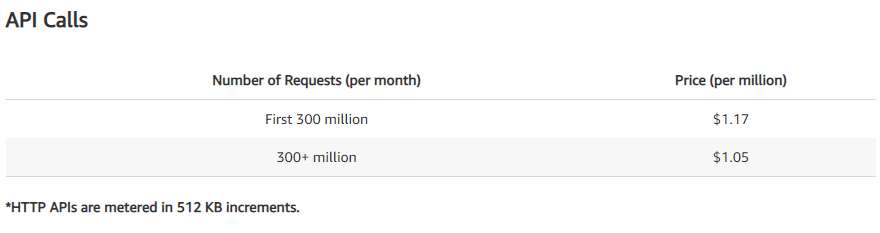
\includegraphics[width=13cm,height=13cm, keepaspectratio]{AWScosts.png}    
    \caption{kosten voor het gebruik van een standaard AWS api gateway \label{awscost}}
\end{figure}

Hieronder valt ook de veranderingen van technologieën.

\section{Het sociale aspect}

In dit hoofdstuk worden de effecten of veranderingen die aan de transformatie verbonden zijn besproken. Deze effecten kunnen zowel positief als negatief zijn, bedoeld of onbedoeld, direct of indirect.

\subsection{Personeel}

De transformatie van een monoliet naar microservices kan een impact hebben op de dagelijkse activiteiten. Tijdens de transformatie kan er gekozen worden voor een nieuwe technologie en kan de systeem infrastructuur aanpassen. Uit het onderzoek van ~\autocite{Schaik2014} blijkt dat er meer weerstand is op complexe veranderingen.  

Hoe duidelijker de verandering is, hoe minder weerstand er zal geboden worden tegen deze verandering.

Omscholing zal ook geld en tijd kosten. Sommige bedrijven willen investeren in hun personeel en bieden hen de kans aan om kennis op te doen over de nieuwe technologie. Deze investering garandeert geen succes.

Verandering zal niet altijd iedereen kunnen overtuigen. De idealen van personen kunnen niet meer in dezelfde lijn liggen als die van het bedrijf. In sommige gevallen kan dit leiden tot een scheiding tussen de twee partijen.

\subsection{Activiteiten}

Tijdens en vooral na de transformatie, zullen de dagelijkse activiteiten van het personeel er anders uit zien. Teams kunnen onderverdeeld worden in kleinere teams die verantwoordelijk zijn voor één of meerdere microservices. Er kunnen nieuwe functies of rollen ontstaan, maar ook bestaande functies kunnen verdwijnen.  

\section{Overzicht}

De overgang van een monolithische architectuur naar microservices zorgt voor vele uitdagingen. Het bedrijf zal een goede schatting moeten maken van de financiële kosten. Een dergelijke transformatie creëert op korte termijn weinig bedrijfswaarde. De kosten zullen stijgen waarbij de winsten op korte termijn niet direct omhoog zullen gaan. Aandeelhouders kunnen daarom niet altijd overtuigd worden om een dergelijke verandering uit te voeren.

Het opgemaakte model bestaat uit vijf pijlers
\begin{itemize}
    \item Tijd
    \item loonkost
    \item infrastructuur
    \item personeel
    \item activiteiten
\end{itemize}

Een bedrijf kan deze vijf pijlers als basis gebruiken om in te schatten wat de mogelijke impact zal zijn van de transformatie.


%%=============================================================================
%% Use case
%%=============================================================================

\chapter{usecase}
\label{ch:usecase}

\section{Inleiding}

In dit hoofdstuk wordt er aan de hand van de verzamelde kennis en het vooropstelde model een bedrijfssituatie geanalyseerd en besproken. Het bedrijf dat onder de loep genomen wordt, is TUI. Het bedrijf is al enkele jaren bezig met de overschakeling van een monolithische architectuur naar microservices. 

Eerst bespreken we waarom het bedrijf wilt veranderen van architectuur. Elk bedrijf heeft een ander doel die ze willen verwezenlijken bij een dergelijke transformatie. Het definiëren van dit doel heeft context rond de beslissingen die genomen werden.

Vervolgens wordt het model uit hoofdstuk \ref{ch:model} toegepast en worden de verschillende aspecten van de transformatie geanalyseerd.

Daarna wordt de manier waarop het proces verloopt, beschreven. Enkele voorbeelden van microservices worden bekeken en wordt er inzicht gegeven over hoe componenten afgesplitst worden van de monoliet. 

Tenslotte is er een overzicht van de gevolgen van deze transformatie.

\subsection{Doel en verwachtingen van de transformatie}

Zoals eerder vermeld is het doel van elk bedrijf anders. In dit geval is het doel van de transformatie om het online platform van TUI te versterken en flexibeler te maken in de steeds wijzigende toerisme sector. Een bijkomend doel is om de verschillende markten (België, Duitsland, Nederland, Engeland, Zweden, Noorwegen, Finland, Denemarken, Oostenrijk, Zwitserland en Ierland) samen te brengen in één platform. TUI heeft namelijk voor elke land een apart systeem, website en database. Het is dus niet enkel een transformatie van een monolithische architectuur naar microservices, maar het is ook de bedoeling dat verschillende systemen samengevoegd worden tot één geheel. Met andere worden is het de bedoeling om meerdere monolieten te transformeren tot één geheel van microservices.  

\subsection{Toepassing van het model}

Volgens het model wordt de impact opgedeeld in vijf pijlers:

\begin{itemize}
    \item \textbf{Tijd}: Het project is begonnen in 2020 en is nog altijd bezig. De eerste mijlsteen werd afgeleverd in 2021 en de tweede mijlsteen is voorzien begin 2022. Het doel is om eind 2023 het project af te werken. Er zijn doelen opgesteld maar slechts enkele werden op tijd opgeleverd. Dit is geen uitzondering voor projecten van deze omvang en complexiteit, maar dit zorgt voor veel extra kosten die niet voorzien waren. Arbeidscontracten die niet voorzien zijn op vertragingen, kunnen heel wat roet in het eten gooien. 
    \item \textbf{Loonkost}: In 2021 waren er tussen de 500 en 1000 mensen die werkten aan de transformatie. Dit zijn ontwikkelaars, testers, \emph{product owners}, ... . Omdat de personen die mee werken aan het project afkomstig zijn uit verschillende landen, is het moeilijk om precies te weten wat de totale loonkost is. 
    \item \textbf{Infrastructuur} : Elke markt heeft zijn eigen infrastructuur. Na de transformatie zou het merendeel gebruik moet maken van de AWS services. Uiteindelijk zou dit de kosten moeten verlagen. Mits er pas overgeschakeld wordt naar het nieuwe systeem na de transformatie, is er tijdens het project een overlap. Zolang het nieuwe systeem niet klaar is, moet het huidige systeem werkend blijven. Dit zorgt voor extra kosten tijdens het project.
    \item \textbf{Personeel} : De transformatie heeft ook een hele grote impact op het personeel. Nationale teams werden internationale teams. De mix van culturen in één team is niet altijd even eenvoudig. Het uurverschil tussen de Europese landen en India zorgt voor een extra drempel. Sommige personeelsleden voelden zich niet meer thuis in deze situatie en kozen voor een nieuwe uitdaging. 
    \item \textbf{Activiteiten} : Voor de transformatie bestonden de meeste activiteiten uit onderhoudstaken voor het \emph{legacy} systeem. Het personeel dat ingezet wordt op de transformatie ontwikkelen microservices. Dit is een groot contrast met de originele activiteiten. Voor sommige personen was dit een verbetering, voor anderen minder.
    
\end{itemize}

\subsection{Verloop van de transformatie}

TUI maakt gebruik van het \emph{Strangler pattern} om hun monoliet stapsgewijs te transformeren naar microservices, zie \ref{ch:stand-van-zaken} voor meer informatie.

Een voorbeeld hiervan is het loskoppelen van de service die informatie biedt aan \emph{Online Travel Agents} van de API.

In de monoliet is deze service onderdeel van de API. Dit houdt in dat wanneer er een aanpassing nodig was specifiek voor \emph{Online Travel Agents}, het volledige deploy proces van de API uitgevoerd moest worden.

\begin{figure}[!htb]
    \centering
    \includegraphics[height=9cm]{tuiflow.png}
    \caption{Tui monoliet \label{tuiflow}}
\end{figure}

In een microservice architectuur is deze service los gekoppeld van de API. De service bestaat uit een API \emph{gateway} en verschillend lambda's. Deze service heeft ook een afzonderlijke \emph{pipeline} voor \emph{deployment}. In de monoliet werd enkel PHP gebruikt voor deze service. Voor de microservice worden er verschillende technologieën en frameworks gebruikt. Om de AWS services automatisch te creëren wordt er gebruikt gemaakt van Terraform. De lambda's zijn geschreven in nodeJS of Python. 

\begin{figure}[!htb]
    \centering
    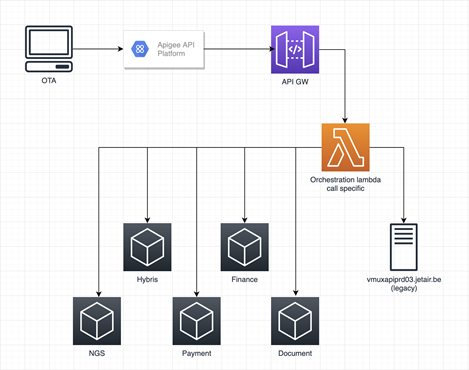
\includegraphics[height=10cm]{OTA.png}
    \caption{Tui microservice \label{tuimicro}}
\end{figure}

Een tweede voorbeeld hiervan is een \emph{micro-frontend}. De oorspronkelijke website was ontwikkeld in Drupal 7. Tijdens de transformatie werd er gekozen om de website te maken in Hybris aangevuld door React - en webcomponenten. De React componenten werden uiteindelijk opgesplitst in micro-frontends. Dit voorbeeld gaat over het prijsoverzicht die de klant te zien krijgt. Deze component is groot genoeg om zelfstandig te functioneren. 

In de oorspronkelijke website was deze module een onderdeel van de website, wat ervoor zorgde dat bij een verandering aan dit component, de volledige website \emph{gedeployed} moest worden.

\begin{figure}[!htb]
    \centering
    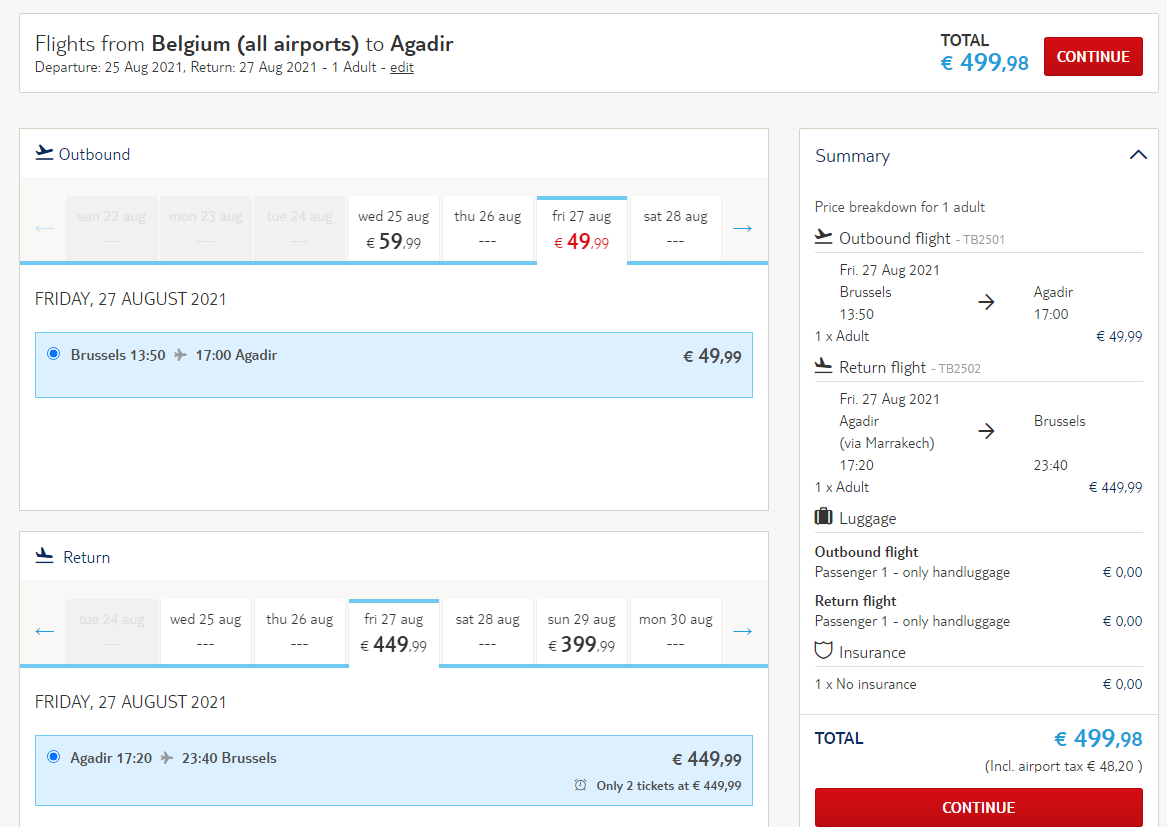
\includegraphics[height = 10cm]{priceSummary-legacy.png}
    \caption{Prijs ovezicht in de monoliet \label{pricelegacy}}
\end{figure}

Als micro-frontend is deze component losgekoppeld van de website en functioneert als een zelfstandig, geisoleerd element. Ook deze micro-frontend wordt gehost op AWS en gebruikt meerdere technologieëen. React, Javascript en Terraform.

\begin{figure}[!htb]
    \centering
    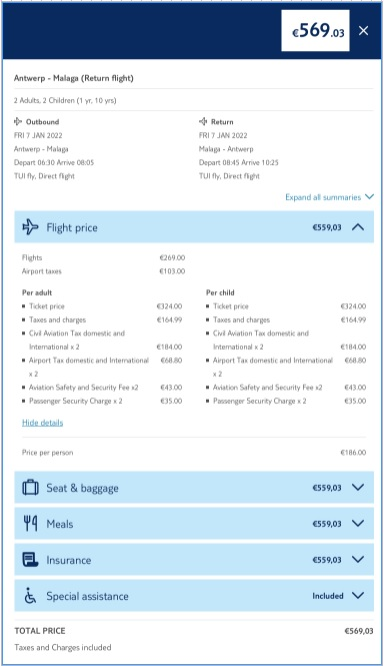
\includegraphics[height = 10cm]{PriceSummaryMicro.jpg}
    \caption{Prijs ovezicht als mircro-frontend \label{pricemicro}}
\end{figure}

\subsection{Gevolgen}

Financieel wordt er heel wat geinvesteerd in het concept van microservices en of de transformatie een succes wordt, is nog niet geweten. Deze overgang vond plaats tijdens covid-19 epidemie en de verkoop van TUI lag zo goed als stil. In theorie zou deze overgang naar microservices TUI sterker moeten maken. Het zou hun online platform een boost kunnen geven op vlak van flexbiliteit en schaalbaarheid. Voorlopig is er nog veel werk voor de boeg. Er moeten nog heel wat problemen opgelost worden en de performance moet nog verbeterd worden, zo niet zal dit project een financiële krater na laten.

In eigen land was het moeilijk om voor een bepaalde prijs het nodige personeel te vinden. Daarom werd er gekozen voor consultants van landen zoals India. Goedkope werkkrachten zorgen niet altijd voor de beste oplossingen.  

De vrijheid in keuze van technologie die microservice biedt, geven meer mogelijkheden. Dit is een stap vooruit, maar het gebruik ervan is nog niet optimaal. 

In theorie is een microservice-architectuur de beste keuze voor TUI. Maar het overgangsproces loopt niet zo vlot als verwacht en er is nog een lange weg te gaan.


% Voeg hier je eigen hoofdstukken toe die de ``corpus'' van je bachelorproef
% vormen. De structuur en titels hangen af van je eigen onderzoek. Je kan bv.
% elke fase in je onderzoek in een apart hoofdstuk bespreken.

%\input{...}
%\input{...}
%...

%%=============================================================================
%% Conclusie
%%=============================================================================

\chapter{Conclusie}
\label{ch:conclusie}

% TODO: Trek een duidelijke conclusie, in de vorm van een antwoord op de
% onderzoeksvra(a)g(en). Wat was jouw bijdrage aan het onderzoeksdomein en
% hoe biedt dit meerwaarde aan het vakgebied/doelgroep? 
% Reflecteer kritisch over het resultaat. In Engelse teksten wordt deze sectie
% ``Discussion'' genoemd. Had je deze uitkomst verwacht? Zijn er zaken die nog
% niet duidelijk zijn?
% Heeft het onderzoek geleid tot nieuwe vragen die uitnodigen tot verder 
%onderzoek?

\lipsum[76-80]



%%=============================================================================
%% Bijlagen
%%=============================================================================

\appendix
\renewcommand{\chaptername}{Appendix}

%%---------- Onderzoeksvoorstel -----------------------------------------------

\chapter{Onderzoeksvoorstel}

Het onderwerp van deze bachelorproef is gebaseerd op een onderzoeksvoorstel dat vooraf werd beoordeeld door de promotor. Dat voorstel is opgenomen in deze bijlage.

% Verwijzing naar het bestand met de inhoud van het onderzoeksvoorstel
%---------- Inleiding ---------------------------------------------------------

\section{Introductie} % The \section*{} command stops section numbering
\label{sec:introductie}

%Hier introduceer je werk. Je hoeft hier nog niet te technisch te gaan.

%Je beschrijft zeker:

%\begin{itemize}
  %\item de probleemstelling en context
  %\item de motivatie en relevantie voor het onderzoek
  %\item de doelstelling en onderzoeksvraag/-vragen
%\end{itemize}

De term 'Microservices' werd voor het eerst gebruikt in een evenement voor software architecten in 2011.
Deze benaming beschrijft een stijl van architectuur, die in die tijd nog in de kinderschoenen stond. Amazon en Netflix waren de pioniers van deze stijl. Deze vorm van architectuur wordt elk jaar populairder dankzij haar flexibiliteit.\\
monolitische systemen zijn grote en vaak complexe gehelen die onderling met elkaar verbonden zijn. Deze structuur vertegenwoordigd nog altijd het merendeel van de bedrijfssystemen. Hiervoor wordt meestal niet bewust gekozen maar is het resultaat van beslissingen op bedrijfsniveau.\\
Oudere bedrijven ondervinden steeds vaker de limieten van de monolitische systemen waardoor ze willen overschakelen naar de flexibelere microservices. Maar is dit wel altijd de juiste keuze? Is er wel genoeg kennis om deze overstap te maken? Hoe lang zal de transformatie duren? Is er genoeg budget? Kortom er zijn heel wat vragen die beantwoord moeten worden.
  

 

%---------- Stand van zaken ---------------------------------------------------

\section{State-of-the-art}
\label{sec:state-of-the-art}

\subsection{Monolitische systemen}
Een monolitische systeem is een architecturale stijl of een softwareontwikkelingspatroon. Vaak zijn het grote en complexe systemen die alle functionaliteit bevatten om aan de noden van de business te voldoen. De logheid is historisch gegroeid: door wijzigingen op wijzigingen. Hierdoor is het moeilijker te onderhouden en vatbaar voor fouten.
~\autocite{Monolith2014}

\subsection{Microservices}
Een microservice is een enkele applicatie die bestaat uit een reeks kleine services, die elk hun eigen proces draaien. Deze processen communiceren met 'light-weight' mechanismen, hoofdzakelijk een API. De services zijn onafhankelijk bruikbaar door volledig geautomatiseerde implementatiemachines. 
~\autocite{Microservices2014}

%---------- Methodologie ------------------------------------------------------
\section{Methodologie}
\label{sec:methodologie}

Als eerste stap zal er een grondige literatuurstudie uitgevoerd worden. In deze studie zullen verschillende aspecten van microservices en monolitische systemen behandeld worden. Het onderzoek zal op basis van volgende sleutelwoorden gestart worden: holacracy, continuous delivery, domain-Driven design, serverless, API, REST, sockets, TCP, gateway, circuit breakers, load balancer en proxy. ~\autocite{Glen2018} ~\autocite{Alshuqayran2016}
Indien er te weinig informatie uit de literatuurstudie gepuurd wordt, zal er een enquête afgenomen worden bij bedrijven die een dergelijke transformatie achter de rug hebben of er volop mee bezig zijn.\\
Aan de hand van de opgedane kennis wordt er een grondig vergelijking uitgevoerd tussen de twee architecturen. Vervolgens wordt er een model opgesteld die gebruikt kan worden om een inschatting te maken over alle mogelijke gevolgen van een transformatie van een monolitische structuur naar een systeem bestaande uit microservices. Het model zal informatie bevatten over volgende criteria:
\begin{itemize}
    \item duur
    \item financiële aspect
    \item vereiste kennis
    \item haalbaarheid
    \item schaalbaarheid
    \item beschikbaarheid
    \item onderhoudbaarheid
    \item ROI
\end{itemize} 
Tenslotte zal het opgestelde model getest worden in verschillend scenario’s waarbij een conclusie genoteerd wordt.

%---------- Verwachte resultaten ----------------------------------------------
\section{Verwachte resultaten}
\label{sec:verwachte_resultaten}

De verwachte resultaten hangen hoofdzakelijk af van de grootte van het bestaande systeem. Hoe groter de monoliet, hoe meer microservices er nodig zullen zijn. Dit geldt voor de meeste criteria die onderzocht zullen worden.\\
De duur van de transformatie hangt af van de grootte en de complexiteit. Diep in elkaar geneste programma's zullen meer tijd nodig hebben.\\
De kostprijs zal beïnvloed worden door verschillende factoren. Als er intern niet genoeg kennis aanwezig is, dan zal het bedrijf externe krachten moeten aanwerven. Een andere mogelijkheid is om te investeren in het huidige personeel. Ondertussen moet ook het bestaande systeem onderhouden worden.

%---------- Verwachte conclusies ----------------------------------------------
\section{Verwachte conclusies}
\label{sec:verwachte_conclusies}
Dit onderzoek zou een verduidelijking moeten geven op de impact van de transformatie van een monolitische systeem naar microservices. Op papier hebben microservices de meeste voordelen ten opzichte van de monolieten, maar deze voordelen zullen niet in iedere situatie opwegen tegen de kosten van de transformatie. Kleinere systemen zullen minder voordeel halen uit het feit dat elke functionaliteit van hun systeem geïsoleerd is. 
Hopelijk kan er een model opgesteld worden die kan voorspellen voor welke situatie de beste architectuur is.



%%---------- Andere bijlagen --------------------------------------------------
% TODO: Voeg hier eventuele andere bijlagen toe
%\input{...}

%%---------- Referentielijst --------------------------------------------------


\end{document}
